\documentclass{article}[a4paper, 12pt]
\usepackage[left=1in,right=1in,top=1.25in,bottom=1.25in]{geometry}
\usepackage{ctex}
\usepackage{amsthm}
\usepackage{hyperref}
\usepackage{amsmath}
\usepackage{amssymb}
\usepackage{tikz}
\usepackage{pgfplots}
\usepackage{unicode-math}
\usetikzlibrary{arrows.meta}
\pgfplotsset{compat=1.17}

\newtheoremstyle{mystyle}
  {1em} % Space above
  {1em} % Space below
  {} % Body font
  {} % Indent amount
  {\bfseries} % Theorem head font
  {.} % Punctuation after theorem head
  {.5em} % Space after theorem head
  {} % Theorem head spec (can be left empty, meaning ‘normal’)

\theoremstyle{mystyle}
\newtheorem{problem}{题}
\newtheorem*{remark}{注记}
\newenvironment{solution}{\begin{proof}[解]}{\end{proof}}

\begin{document}

\title{复分析第五次习题课}
\author{彭子鱼}
\date{2024 年 5 月 26 日\\上次更新: \today}

\maketitle

\section{作业}

\begin{problem}[5.1.2]
  求函数在给定域上的Laurent展开.
  \begin{itemize}
    \item[(1)] \(\frac{1}{z^2(z-1)}\), \(D=B(1,1)\backslash\{1\}\);
    \item[(3)] \(\text{Log}\left(\frac{z-1}{z-2}\right)\), \(D=B(\infty,2)\);
    \item[(5)] \(\frac{1}{(z-5)^n}\), \(n\ge0\), \(D=B(\infty,5)\).
  \end{itemize}
\end{problem}

\begin{solution}
  \begin{itemize}
    \item [(1)] 由于\(|z-1|<1\), \[\begin{aligned}
      \frac{1}{z^2(z-1)}&=\frac{1}{z-1}\cdot\frac{1}{(1+z-1)^2}\\
      &=\frac{1}{z-1}\cdot\sum_{n=0}^\infty (-1)^n(n+1)(z-1)^n\\
      &=\sum_{n=0}^\infty (-1)^n(n+1)(z-1)^{n-1}.
    \end{aligned}\]
    \item [(3)] 易验证在\(B(\infty,2)\)上\(\text{Log}\left(\frac{z-1}{z-2}\right)\)可取出单值全纯分支, 只需考虑主支. \[\begin{aligned}
      \log\left(\frac{z-1}{z-2}\right)&=\log\left(1-\frac1z\right)-\log\left(1-\frac2z\right)\\
      &=-\sum_{n=1}^\infty \frac{1}{nz^n}+\sum_{n=1}^\infty\frac{2^n}{nz^n}\\
      &=\sum_{n=1}^\infty \frac{2^n-1}{n}z^{-n}.
    \end{aligned}\]
    故\[\text{Log}\left(\frac{z-1}{z-2}\right)=\sum_{n=1}^\infty \frac{2^n-1}{n}z^{-n}+2k\pi i,\] 其中\(k\in\mathbb{Z}\).
    \item [(5)] 由于\(|\frac{5}{z}|<1\), \begin{align*}
      \frac{1}{(z-5)^n}&=\frac{1}{z^n}\frac{1}{(1-\frac{5}{z})^n}\\
      &=\frac{1}{z^n}\sum_{k=0}^\infty \frac{1}{k!}n(n+1)\cdots(n+k-1)\left(\frac{5}{z}\right)^k\\
      &=\sum_{k=0}^\infty \binom{n+k-1}{n-1}5^kz^{-n-k}. \tag*{\(\qed\)}
    \end{align*}
  \end{itemize}
  \renewcommand{\qedsymbol}{}
\end{solution}

\begin{remark}
  求Laurent级数时, 须注意在何处展开.
\end{remark}

\begin{problem}[5.2.2]
  求函数\(f(z)\)的奇点并判断其类型.
  \begin{itemize}
    \item [(3)] \(\sin\frac{1}{z-1}\);
    \item [(7)] \(\sin\left(\frac{1}{\cos\frac{1}{z}}\right)\);
    \item [(8)] \(e^{\tan z}\).
  \end{itemize}
\end{problem}

\begin{solution}
  \begin{itemize}
    \item [(3)] 可能的奇点为\(1,\infty\). 因为\(\lim\limits_{z\to1}f(z)\)不存在, \(\lim\limits_{z\to0}f\left(\frac{1}{z}\right)=\lim\limits_{z\to0}\sin\frac{z}{z-1}=0\), 所以\(1\)是本性奇点, \(\infty\)是可去奇点.
    \item [(7)] 可能的奇点为\(0,\infty,\frac{2}{(2k+1)\pi}\), 其中\(k\in\mathbb Z\). 因为\(\lim\limits_{z\to\frac{2}{(2k+1)\pi}}f(z)\)不存在, 所以\(\frac{2}{(2k+1)\pi}\) (\(k\in\mathbb Z\))是本性奇点. 从而\(0\)是非孤立奇点. 因为\(\lim\limits_{z\to 0}f\left(\frac{1}{z}\right)=\lim\limits_{z\to 0}\sin\left(\frac{1}{\cos z}\right)=\sin 1\), 所以\(\infty\)是可去奇点.
    \item [(8)] 可能的奇点为\(\infty, k\pi+\frac\pi2\), 其中\(k\in\mathbb Z\). 因为\(\lim\limits_{z\to k\pi+\frac\pi2}f(z)\)不存在, 所以\(k\pi+\frac\pi2\) (\(k\in\mathbb Z\))是本性奇点. 从而\(\infty\)是非孤立奇点. \qedhere
  \end{itemize}
\end{solution}

\begin{remark}
  须讨论\(\infty\)的类型. 注意非孤立奇点的概念.
\end{remark}

\begin{problem}[5.3.1]
  求所有\(\mathbb C\)上亚纯函数\(f\), 使得\(|f(z)|=1\)对任意\(z\in\partial B(0,1)\)成立.
\end{problem}

\begin{solution}
  由\(f\)亚纯且非零, 其在\(B(0,1)\)只有有限个零点和极点, 设\(f\)零点为\(z_1,\dots,z_n\), 极点为\(w_1,\dots,w_m\) (可重复). 

  令\[g(z)=f(z)\prod_{k=1}^{n}\frac{1-\bar{z}_kz}{z-z_k}\prod_{l=1}^{m}\frac{z-w_l}{1-\bar{w}_lz},\] 则\(g\)在\(\overline{B(0,1)}\)全纯且无零点, \(|g(z)|=1\)对任意\(z\in\partial B(0,1)\)成立. 考虑\(\frac1g\)并利用最大模原理, \(g\)为常数, 即\(g(z)=e^{i\theta}\), \(\theta\in\mathbb R\).

  故所有满足要求的函数为\[f(z)=e^{i\theta}\prod_{k=1}^{n}\frac{z-z_k}{1-\bar{z}_kz}\prod_{l=1}^{m}\frac{1-\bar{w}_lz}{z-w_l},\] 其中\(\theta\in\mathbb R\), \(n,m\)为非负整数, \(z_1,\dots,z_n,w_1,\dots,w_m\in B(0,1)\).
\end{solution}

\begin{problem}[5.4.8]
  求函数的孤立奇点并求出其留数.
  \begin{itemize}
    \item [(6)] \(\sin\frac{z}{z+1}\);
    \item [(8)] \(\frac{e^{\pi z}}{z^2+1}\).
  \end{itemize}
\end{problem}

\begin{solution}
  \begin{itemize}
    \item [(6)] 可能的奇点为\(-1,\infty\). 因为\(\lim_{z\to-1}f(z)\)不存在, 所以\(-1\)是本性奇点. 因为\(\lim_{z\to0}f(\frac{1}{z})=\sin1\), 所以\(\infty\)是可去奇点.
    
    由5.4.3, \[\text{Res}(f,\infty)=\lim_{z\to\infty}z^2f'(z)=\lim_{z\to\infty}\frac{z^2}{(z+1)^2}\cos\frac{z}{z+1}=\cos 1.\]
    由留数定理, \[\text{Res}(f,-1)=-\text{Res}(f,\infty)=-\cos 1.\]
    \item [(8)] 可能的奇点为\(\pm i,\infty\). 因为\(\lim_{z\to \pm i}f(z)=\infty\), 所以\(\pm i\)是极点. 因为\(\lim_{z\to0}f(\frac{1}{z})\)不存在, 所以\(\infty\)是本性奇点.
    
    由\(\pm i\)是1阶极点, \[\text{Res}(f,i)=\lim_{z\to i}(z-i)f(z)=\frac{i}{2},\] \[\text{Res}(f,-i)=\lim_{z\to -i}(z+i)f(z)=-\frac{i}{2}.\]
    由留数定理, \(\text{Res}(f,\infty)=0\). \qedhere
  \end{itemize}
\end{solution}

\begin{problem}[5.4.9]
  设\(f,g\)在\(B(0,R)\)中全纯, 在\(\overline{B(0,R)}\)上连续, \(g\)在\(\partial B(0,R)\)上无零点, \(g\)在\(B(0,R)\)中的全部零点\(z_1,\dots,z_n\)都是1阶零点. 求\[\frac{1}{2\pi i}\int_{|z|=R}\frac{f(z)}{zg(z)}dz.\]
\end{problem}

\begin{solution}
  记\(h(z)=\frac{f(z)}{zg(z)}\).

  先证明: 若\(z_k\ne0\), 则对充分小的\(\varepsilon>0\),\[\frac{1}{2\pi i}\int_{|z-z_k|=\varepsilon}\frac{f(z)}{zg(z)}dz=\frac{f(z_k)}{z_kg'(z_k)}.\] 
  
  这可分两种情况讨论. 若\(f(z_k)\ne 0\), 则\(z_k\)是\(h\)的1阶极点, \[\text{Res}(h,z_k)=\lim_{z\to z_k}\frac{f(z)}{z}\cdot\frac{z-z_k}{g(z)}=\frac{f(z_k)}{z_kg'(z_k)}.\] 若\(f(z_k)=0\), 则\(z_k\)是\(h\)的可去奇点, 从而\(\int_{|z-z_k|=\varepsilon}\frac{f(z)}{zg(z)}dz=0\). 总之, 上式成立.

  再讨论\(0\)处情形. 对充分小的\(\varepsilon>0\), 记\[I=\frac{1}{2\pi i}\int_{|z|=\varepsilon}\frac{f(z)}{zg(z)}dz.\]
  
  若\(0\)不是\(g\)的零点, 则\(0\)是\(h\)的1阶极点或可去奇点, 由\(f(0)\)是否为0决定. 和上面类似可知\[I=\frac{f(0)}{g(0)}.\]

  若\(0\)是\(g\)的零点, 对\(f\)在0处情况讨论. \newline 若\(0\)是\(f\)的至少2阶零点, 则\(0\)是\(h\)的可去奇点, 从而\[I=0.\] 若\(0\)是\(f\)的1阶零点, 则\(0\)是\(h\)的1阶极点, \[I=\text{Res}(h,0)=\lim_{z\to0}zh(z)=\lim_{z\to0}\frac{f(z)/z}{g(z)/z}=\frac{f'(0)}{g'(0)}.\] 若\(0\)不是\(f\)的零点, 则\(0\)是\(h\)的2阶极点, \[I=\text{Res}(h,0)=\lim_{z\to0}(z^2h(z))'=\lim_{z\to0}\left(\frac{zf(z)}{g(z)}\right)'=\frac{f'(0)}{g'(0)}-\frac{f(0)g''(0)}{2(g'(0))^2}.\]

  由Cauchy积分定理, \[\frac{1}{2\pi i}\int_{|z|=R}\frac{f(z)}{zg(z)}dz=I+\sum_{k=1}^n\frac{1}{2\pi i}\int_{|z-z_k|=\varepsilon}\frac{f(z)}{zg(z)}dz.\] 故\[\frac{1}{2\pi i}\int_{|z|=R}\frac{f(z)}{zg(z)}dz=\sum_{k:z_k\ne0}\frac{f(z_k)}{z_kg'(z_k)}+\frac{f(0)}{g(0)}\mathbb{1}\{g(0)\ne0\}+\left(\frac{f'(0)}{g'(0)}-\frac{f(0)g''(0)}{2(g'(0))^2}\right)\mathbb{1}\{g(0)=0\}.\qedhere\]
\end{solution}

\begin{problem}[5.4.10]
  求积分.
  \begin{itemize}
    \item [(1)] \(\int_{|z|=2}\frac{1}{z^3(z^{10}-2)}dz\);
    \item [(4)] \(\int_{|z|=R}\frac{z^2}{e^{2\pi i z^3}-1}dz\).
  \end{itemize}
\end{problem}

\begin{solution}
  \begin{itemize}
    \item [(1)] 易知\(f\)在\(B(\infty,2)\)上全纯, 且\(\infty\)为可去奇点. 从而\[\text{Res}(f,\infty)=0.\] 故\[\int_{|z|=2}\frac{1}{z^3(z^{10}-2)}dz=-2\pi i\text{Res}(f,\infty)=0.\]
    \item [(4)] 作换元\(w=z^3\). 注意\(z^2dz=\frac13dw\), 换元后变成绕3圈, 二者抵消. 因此\[\int_{|z|=R}\frac{z^2}{e^{2\pi i z^3}-1}dz = \int_{|w|=R^3}\frac{1}{e^{2\pi i w}-1}dw.\]
    
    在\(|w|<R^3\), \(\frac{1}{e^{2\pi i w}-1}\)有1阶极点\(0,\pm1,\dots,\pm n\), 且留数均为\(\frac{1}{2\pi i}\).

    故\[\int_{|z|=R}\frac{z^2}{e^{2\pi i ^3}-1}dz=2\pi i\cdot(2n+1)\cdot\frac{1}{2\pi i}=2n+1. \tag*{\(\qed\)}\]
  \end{itemize}
  \renewcommand{\qedsymbol}{}
\end{solution}

\begin{problem}[5.5.1(8)]
  计算\[I=\int_0^\infty \frac{\cos x}{(1+x^2)^3}dx.\]
\end{problem}

\begin{solution}
  令\(f(z)=\frac{e^{iz}}{(1+z^2)^3}\). 记\(\gamma_R=\{z=Re^{i\theta}:\theta\in[0,\pi]\}\). 由Jordan引理, \[\lim_{R\to\infty}\int_{\gamma_R}f(z)dz=0.\]

  由留数定理, \[\int_{-R}^R f(x)dx+\int_{\gamma_R}f(z)dz=2\pi i\text{Res}(f, i)=2\pi i\lim_{z\to i}\frac{d^2}{dz^2}\frac{e^{iz}}{(z+i)^3}=\frac{7}{8}\pi e^{-1}.\]

  令\(R\to \infty\)并注意\(\frac{\cos x}{(1+x^2)^3}\)是偶函数, 取实部得\[I=\frac{7}{16}\pi e^{-1}.\tag*{\(\qed\)}\]
  \renewcommand{\qedsymbol}{}
\end{solution}

\begin{problem}[5.5.1(9)] \label{9}
  计算\[I=\int_0^\infty \left(\frac{\sin x}{x}\right)^2dx.\]
\end{problem}

\begin{figure}[htbp]
  \centering
  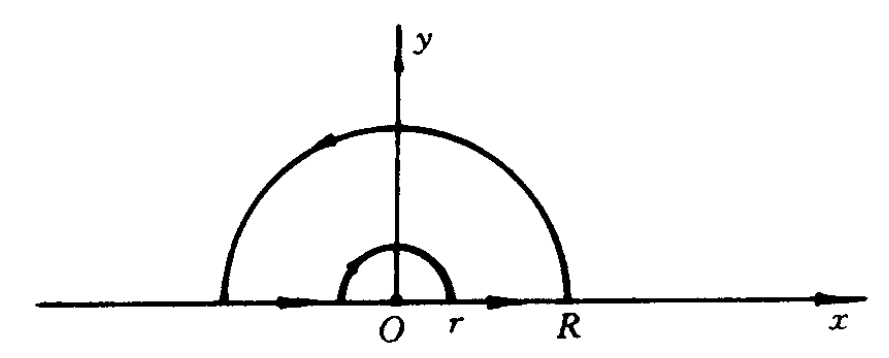
\includegraphics[width=0.8\textwidth]{images/9.png}
  \caption{题\ref{9}的图示.}
  \label{fig:9}
\end{figure}

\begin{solution}
  令\(f(z)=\frac{e^{2iz}-1}{z^2}\). 考虑\ref{fig:9}中围道. 则\[\int_{-R}^{-r}-\int_{\gamma_r}+\int_{r}^R+\int_{\gamma_R} f(z)dz=:I_1-I_2+I_3+I_4=0.\]

  作换元\(x\to -x\), \[I_1+I_3=\int_r^R \frac{e^{-2ix}-1}{x^2}dx+\int_r^R \frac{e^{2ix}-1}{x^2}dx=-4\int_r^R \left(\frac{\sin x}{x}\right)^2dx.\]

  由Jordan引理, \[\lim_{R\to\infty} I_4=0.\]

  由引理5.5.9, \[\lim_{r\to0}I_2=i\pi\lim_{z\to0}zf(z)=-2\pi.\]

  令\(R\to\infty\), \(r\to0\)得\(-4I+2\pi=0\), 即\[I=\frac{\pi}{2}.\tag*{\(\qed\)}\]
  \renewcommand{\qedsymbol}{}
\end{solution}

\begin{problem}[5.5.1(11)]
  计算\[I=\int_0^\infty \frac{x^p}{1+x^2}dx,\] 其中\(-1<p<1\).
\end{problem}

\begin{solution}
  一般地, 
\end{solution}

\begin{problem}[5.5.1(15)]
  计算\[I=\int_0^1 \frac{x^{1-p}(1-x)^p}{1+x^2}dx,\] 其中\(-1<p<2\).
\end{problem}

\begin{problem}[5.5.1(21)]
  计算\[I=\int_0^\infty \frac{\log x}{x^2-1}dx.\]
\end{problem}

\begin{problem}[5.5.1(25)] \label{25}
  计算\[I=\int_0^\infty \frac{x}{e^x+1}dx.\]
\end{problem}

\begin{figure}[htbp]
  \centering
  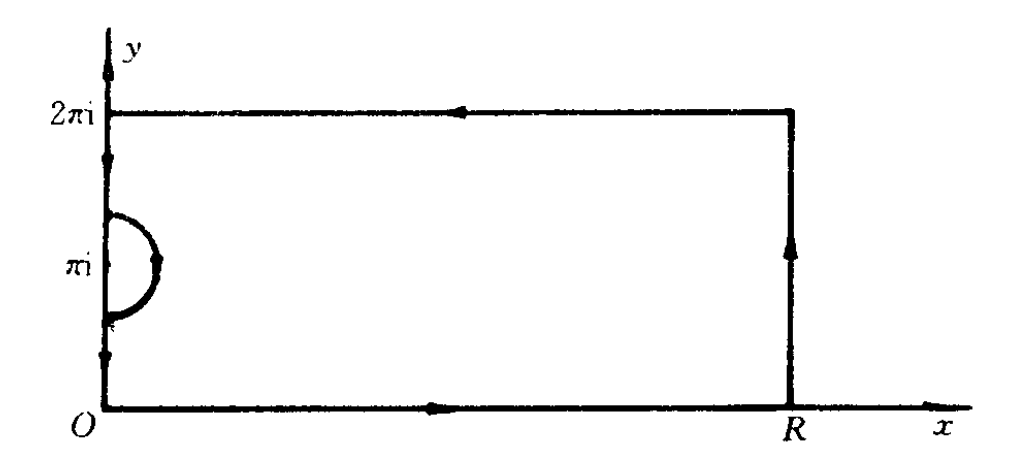
\includegraphics[width=0.8\textwidth]{images/25.png}
  \caption{题\ref{25}的图示.}
  \label{fig:25}
\end{figure}

\begin{solution}
  令\(f(z)=\frac{z^2}{e^z+1}\).
\end{solution}

\end{document}